%!TEX program = xelatex

\documentclass[compress,xcolor=table]{beamer}
%--------------------------------------------------------------------------
% Common packages
%--------------------------------------------------------------------------

\definecolor{links}{HTML}{663000}
\hypersetup{colorlinks,linkcolor=,urlcolor=links}

\usepackage[english]{babel}
\usepackage{pgfpages} % required for notes on second screen
\usepackage{graphicx}

\usepackage{multicol}
\usepackage{multirow}

\usepackage{tabularx,ragged2e}
\usepackage{booktabs}

\setlength{\emergencystretch}{3em}  % prevent overfull lines

\usetheme{hri}
\usetikzlibrary{shapes.geometric}
\usetikzlibrary{svg.path}

% Display the navigation bullet even without subsections
\usepackage{remreset}% tiny package containing just the \@removefromreset command
\makeatletter
\@removefromreset{subsection}{section}
\makeatother
\setcounter{subsection}{1}

\makeatletter
\let\beamer@writeslidentry@miniframeson=\beamer@writeslidentry
\def\beamer@writeslidentry@miniframesoff{%
  \expandafter\beamer@ifempty\expandafter{\beamer@framestartpage}{}% does not happen normally
  {%else
    % removed \addtocontents commands
    \clearpage\beamer@notesactions%
  }
}
\newcommand*{\miniframeson}{\let\beamer@writeslidentry=\beamer@writeslidentry@miniframeson}
\newcommand*{\miniframesoff}{\let\beamer@writeslidentry=\beamer@writeslidentry@miniframesoff}
\makeatother



\newcommand{\source}[2]{{\tiny\it Source: \href{#1}{#2}}}

\usepackage{tikz}
\usetikzlibrary{mindmap,backgrounds,positioning,calc,patterns}

\graphicspath{{figs/}}

\title{Human-Robot Interaction}
\subtitle{Machine Learning for HRI}
\date{}
\author{Séverin Lemaignan}
\institute{{\bf Bristol Robotics Lab}\\University of the West of England}

\begin{document}

\miniframesoff

\licenseframe{github.com/severin-lemaignan/lecture-hri-ml-for-hri}

{
\setbeamercolor{background canvas}{bg=uweBlue}
\maketitle
}


\begin{frame}{In this lecture}

\begin{itemize}
    \item Build your own emotion classifier from scratch!
    \item Basic classifiers: kNNs, SVM, MLP
%    \item What does the state-of-art look like? Deep graph nets, GANs, Attention
%        nets
    \item ML to teach a robot social behaviours

\end{itemize}

\end{frame}

\miniframeson

\section{Emotions?}

\begin{frame}{Paul Ekman and basic emotions}

\href{https://en.wikipedia.org/wiki/Paul_Ekman}{Paul Ekman}, a
psychologist, found that when shown facial expressions people across the
world all recognised six \textbf{basic emotions}.

    \only<1>{
    \begin{center}
        \includegraphics[width=0.55\linewidth]{emotions/ekman_6_basic_emotions}

        \source{http://emotionresearcher.com/}{emotionresearcher.com}
    \end{center}
}

\pause

\begin{center}
\textbf{Anger, disgust, fear, happiness, sadness and surprise}.
\end{center}

\pause 
In 1990 Ekman extended his list of basic emotion to include other
emotions: \emph{Amusement, contempt, contentment, embarrassment, excitement, guilt,
  pride in achievement, relief, satisfaction, sensory pleasure, and
    shame}

    \begin{exampleblock}{Attention}
Ekman's model does not adequately reflect the real-world complexity of emotions.
Today, we favour continuous models like valence-arousal, or
        Pleasure-Arousal-Dominance (PAD), or discuss more general \emph{facial
        expressions}.

\end{exampleblock}

\end{frame}


%
%
%\begin{frame}{How to represent emotions?}
%
%\only<1-4>{
%    Several approaches (or {\bf models}):
%}
%
%\only<1-2>{
%ON/OFF approach to basic emotions:
%
%\begin{itemize}
%
%\item Anger : ON/OFF
%\item Disgust : ON/OFF
%\item Fear : ON/OFF
%\item Happiness : ON/OFF
%\item Sadness : ON/OFF
%\item Surprise : ON/OFF
%\end{itemize}
%
%Why is this a poor approach to representing emotion?
%
%\pause
%
%$\Rightarrow$ no representation of gradual emotions; all is just ``on'' or
%``off''
%}
%\only<3-4>{
%
%
%Gradual representation of emotion would be better:
%
%\begin{itemize}
%
%\item Anger : {[}0; 1{]}
%\item Disgust : {[}0; 1{]}
%\item Fear : {[}0; 1{]}
%\item Happiness : {[}0; 1{]}
%\item Sadness : {[}0; 1{]}
%\item Surprise : {[}0; 1{]}
%\end{itemize}
%
%What is the problem with this representation?
%
%\onslide<4>
%$\Rightarrow$ can lead to contradicting emotion representation, for example
%Happiness = 1 and Sadness = 1.
%}
%
%
%    \only<5>{
%    $\Rightarrow$ continuous representations of emotions in space
%}
%\end{frame}
%
%{
%    \paper{Russell J. {\bf A circumplex model of affect} 1980}
%\begin{frame}{Circumplex model}
%
%Two-dimensional space (\textbf{arousal} and \textbf{valence} on x and y
%dimensions)
%
%\begin{itemize}
%
%\item emotions are noted on circumference of the circle.
%\item middle of circle (0,0) is \textbf{neutral}
%\item the further from the centre, the stronger the emotion.
%\end{itemize}
%
%    \begin{center}
%        \includegraphics[width=0.55\linewidth]{circumplex}
%        \source{http://www.ncbi.nlm.nih.gov/pmc/articles/PMC2367156/}{Posner
%et al., 2005}
%    \end{center}
%\end{frame}
%}
%
%{
%    \paper{Mollahosseini et al. {\bf Affectnet: A database for facial
%    expression, valence, and arousal computing in the wild} 2017}
%\begin{frame}{Circumplex model}
%    \begin{center}
%        \includegraphics[width=0.65\linewidth]{AffectNet_circumplex.png}
%    \end{center}
%\end{frame}
%}
%
%
%\begin{frame}{P-A-D model}
%
%By Albert Mehrabian and James A. Russell (1974)
%
%Three-dimensional representation of emotion.
%
%\begin{itemize}
%
%\item \textbf{Pleasure, Arousal and Dominance}.
%\item Most used model in robotics and Human-Machine Interaction
%\end{itemize}
%
%\pause
%
%\textbf{Pleasure}: how pleasant is an emotion. Anger and fear are
%unpleasant emotions, and score low on the pleasure scale. Joy is a
%pleasant emotion.
%
%\pause
%
%\textbf{Arousal}: intensity of an emotion. Anger and rage are unpleasant
%emotions, but rage has a higher intensity or a higher arousal state.
%However boredom, which is also an unpleasant state, has a low arousal
%value.
%
%\pause
%
%\textbf{Dominance}: controlling and dominant nature of the emotion. For
%instance while both fear and anger are unpleasant emotions, anger is a
%dominant emotion, while fear is a submissive emotion.
%
%\end{frame}
%
%{
%    \paper{H. Hoffmann, A Scheck, T. Schuster, H. Kessler {\bf Mapping discrete
%    emotions into the dimensional space: An empirical approach} 2012}
%\begin{frame}{PAD model}
%
%    \begin{columns}
%        \begin{column}{0.5\linewidth}
%    \begin{center}
%        \includegraphics[width=\linewidth]{pad}
%    \end{center}
%
%
%        \end{column}
%        \begin{column}{0.5\linewidth}
%        \begin{center}
%            \includegraphics[width=\linewidth]{pad-mapping}
%        \end{center}
%        \end{column}
%    \end{columns}
%
%\end{frame}
%}
%
%


\section{Classification}

\begin{frame}{Classification}

Social signal processing often relies on \textbf{classification.}

\begin{itemize}
    \item \href{https://en.wikipedia.org/wiki/Statistical_classification}{\textbf{Classification}}
        is deciding on which \textbf{category} a new observation belongs to
        based on training data.

    \item The training data contains data and known categories.
    \item Classification is a \textbf{supervised} learning algorithm.
\end{itemize}

\pause

Examples:

\scriptsize
\begin{itemize}

\item An incoming tweet needs to classified as being positive or negative.
\item An radar ping of a flying objects needs to be classified as belonging
  to one of \emph{n} possible planes.
\item The prosody of speech needs to be classified as belonging to one of
  six basic categories of emotion (happy, sad, angry, bored, surprised,
  neutral).
\item A gesture filmed through a camera needs to be classified as meaning
  stop, go, left or right.
\end{itemize}

\end{frame}

\begin{frame}{Classification: example}

\begin{itemize}
\item Two dimensional problem
\item Two categories, with training data for both categories
\item To which category does a new observation belong?
\end{itemize}

    \begin{center}
        \resizebox{0.5\linewidth}{!}{
            \begin{tikzpicture}[>=latex,
                starmarker/.style={star, fill=hriSec2Comp,opacity=0.5,inner sep=0,minimum size=4pt}]

                %\draw[help lines] (0,0) grid (5,4);
                \draw[thick, ->] (0,0) -> (5.2,0);
                \draw[thick, ->] (0,0) -> (0,4.2);

                \fill [hriSec2, opacity=0.5] (2.2,1.3) circle (2pt);
                \fill [hriSec2, opacity=0.5] (3.2,2.3) circle (2pt);
                \fill [hriSec2, opacity=0.5] (2.5,0.4) circle (2pt);
                \fill [hriSec2, opacity=0.5] (0.6,0.3) circle (2pt);
                \fill [hriSec2, opacity=0.5] (2.8,0.7) circle (2pt);
                \fill [hriSec2, opacity=0.5] (3.8,1.7) circle (2pt);
                \fill [hriSec2, opacity=0.5] (4.5,1.0) circle (2pt);

                \only<1-2,4->{
                    \fill [hriSec2, opacity=0.5] (4.1,2.4) circle (2pt);
                    \fill [hriSec2, opacity=0.5] (4.5,3.5) circle (2pt);
                }

                \fill [hriSec3Comp, opacity=0.5] (2.3,3.2) rectangle +(3.5pt,3.5pt);
                \fill [hriSec3Comp, opacity=0.5] (0.3,0.6) rectangle +(3.5pt,3.5pt);
                \fill [hriSec3Comp, opacity=0.5] (1.5,1.4) rectangle +(3.5pt,3.5pt);
                \fill [hriSec3Comp, opacity=0.5] (2.4,2.2) rectangle +(3.5pt,3.5pt);
                \fill [hriSec3Comp, opacity=0.5] (0.7,2.8) rectangle +(3.5pt,3.5pt);
                \fill [hriSec3Comp, opacity=0.5] (1.7,3.8) rectangle +(3.5pt,3.5pt);
                \fill [hriSec3Comp, opacity=0.5] (1.0,2.5) rectangle +(3.5pt,3.5pt);

                \only<1-3>{
                    \fill [hriSec3Comp, opacity=0.5] (2.2,2.5) rectangle +(3.5pt,3.5pt);
                    \fill [hriSec3Comp, opacity=0.5] (1.3,2.2) rectangle +(3.5pt,3.5pt);
                }
                \only<4->{
                    \fill [hriSec2, opacity=0.5] (2.2,2.5) circle (2pt);
                    \fill [hriSec2, opacity=0.5] (1.3,2.2) circle (2pt);
                }


                \only<1>{
                    \fill (3.5,3) circle (2pt) node[above] {?};
                }

                \only<2>{
                    \draw[dashed, ultra thick] (0,0.1) -- (4.9,4);
                    \fill[hriSec3Comp] (3.5,3) circle (3pt);
                }

                \only<3->{
                \node[starmarker] at(2.8,3.5) {};
                \node[starmarker] at(3.2,2.6) {};
                \node[starmarker] at(3.7,2.5) {};
                \node[starmarker] at(4.8,2.3) {};
                \node[starmarker] at(4.2,3.5) {};
                \node[starmarker] at(4.7,3.2) {};
                \node[starmarker] at(3.6,3.5) {};
                \node[starmarker] at(3.2,3.0) {};
            }

                \only<3>{
                \coordinate (center) at (3,2.5);
                    \draw[dashed, ultra thick] (0,0.1) -- (center);
                    \draw[dashed, ultra thick] (2.1,4) -- (center);
                    \draw[dashed, ultra thick] (5,2) -- (center);
                }

                \only<4>{
                    \draw[ultra thick, dashed] svg[scale=0.355mm] {M 0,0 C 7.3028978,5.4871928 17.986558,18.924336 25.712718,23.631806 33.180198,27.981126 42.096418,29.772386 48.918988,35.157436 53.234728,39.486306 53.152318,48.037756 47.022748,50.669426 42.040828,52.174296 36.443098,53.302996 33.138128,57.811566 29.262578,61.437306 31.018648,68.735086 36.313848,69.650946 45.513978,70.336506 52.317528,79.815856 61.890318,78.092016 67.994798,76.405086 66.315798,68.913296 65.206548,64.346256 62.816378,59.430726 65.265748,53.196516 71.506418,55.666566 76.735423,57.642746 77.207603,62.923806 82.494663,67.005556 87.781723,71.087306 97.769793,65.300896 103.85227,64.480036 109.93475,63.659176 113.08322,69.782766 115.38846,74.251266 119.51535,82.521786 120.32667,91.925786 123.66302,100.4599 126.136,107.56288 135.65151,102.31662 131.03155,96.353476 128.47853,90.355456 123.56513,84.297766 125.88953,77.387966 127.40319,68.340166 132.79437,57.935476 141.71719,53.730616};
                    \draw[ultra thick, dashed] svg[scale=0.355mm] {M 84.116373,67.870526 C 84.388083,71.283156 84.773743,74.838716 83.492033,78.110256 82.006413,83.150896 79.611653,88.027626 75.899043,91.805036 73.482483,94.619536 71.510448,97.822816 70.142548,101.27341 69.330828,105.09004 70.025558,108.99486 70.135548,112.8405};
                }



            \end{tikzpicture}
        }
    \end{center}


    \only<2> {
        When categories can be linearly separated, we have a very easy
        classification problem.
    }

    \only<3> {
        Three or more can still be linearly separated.
    }


    \only<4-> {
        \textbf{But what if categories are not linearly separable?}
    }

\end{frame}

\begin{frame}{Three classification methods}

Three methods will be explained here:

\begin{itemize}

\item $k$-nearest Neighbours (kNN)
\item Support Vector Machines (SVM)
\item Multi-layer perceptrons (MLP)
\end{itemize}

    {\scriptsize
Many other classifiers are possible
    (\href{https://scikit-learn.org/stable/auto_examples/classification/plot_classifier_comparison.html}{\scriptsize
    Comparison of classifiers with scikit-learn}):

\begin{itemize}

\item Decision trees/Random forest
\item Bayes classifiers
\item The large family of neural networks (MLP is the simplest one)
\item \ldots{}
\end{itemize}
    }

    \begin{center}
        \includegraphics[width=0.8\linewidth]{figs/sklearn-classifiers.png}
    \end{center}

\end{frame}

\begin{frame}{$k$-nearest Neighbours}


When an observation comes in, calculate the distance to the $k$ nearest
neighbours. The observation belongs to the class the most frequent amongst neighbours.

    \begin{center}
        \resizebox{0.5\linewidth}{!}{
            \begin{tikzpicture}[>=latex,
                starmarker/.style={star, fill=hriSec2Comp,opacity=0.5,inner sep=0,minimum size=4pt}]

                %\draw[help lines] (0,0) grid (5,4);
                \draw[thick, ->] (0,0) -> (5.2,0);
                \draw[thick, ->] (0,0) -> (0,4.2);

                \fill [hriSec2, opacity=0.5] (2.2,1.3) circle (2pt);
                \fill [hriSec2, opacity=0.5] (3.2,2.3) circle (2pt);
                \fill [hriSec2, opacity=0.5] (2.5,0.4) circle (2pt);
                \fill [hriSec2, opacity=0.5] (0.6,0.3) circle (2pt);
                \fill [hriSec2, opacity=0.5] (2.8,0.7) circle (2pt);
                \fill [hriSec2, opacity=0.5] (3.8,1.7) circle (2pt);
                \fill [hriSec2, opacity=0.5] (4.5,1.0) circle (2pt);

                \fill [hriSec2, opacity=0.5] (1.3,2.2) circle (2pt);
                \fill [hriSec2, opacity=0.5] (4.1,2.4) circle (2pt);
                \fill [hriSec2, opacity=0.5] (4.5,3.5) circle (2pt);
                \fill [hriSec2, opacity=0.5] (2.2,2.5) circle (2pt);

                \fill [hriSec3Comp, opacity=0.5] (2.3,3.2) rectangle +(3.5pt,3.5pt);
                \fill [hriSec3Comp, opacity=0.5] (0.3,0.6) rectangle +(3.5pt,3.5pt);
                \fill [hriSec3Comp, opacity=0.5] (1.5,1.4) rectangle +(3.5pt,3.5pt);
                \fill [hriSec3Comp, opacity=0.5] (2.4,2.2) rectangle +(3.5pt,3.5pt);
                \fill [hriSec3Comp, opacity=0.5] (0.7,2.8) rectangle +(3.5pt,3.5pt);
                \fill [hriSec3Comp, opacity=0.5] (1.7,3.8) rectangle +(3.5pt,3.5pt);
                \fill [hriSec3Comp, opacity=0.5] (1.0,2.5) rectangle +(3.5pt,3.5pt);



                \node[starmarker] at(2.8,3.5) {};
                \node[starmarker] at(3.2,2.6) {};
                \node[starmarker] at(3.7,2.5) {};
                \node[starmarker] at(4.8,2.3) {};
                \node[starmarker] at(4.2,3.5) {};
                \node[starmarker] at(4.7,3.2) {};
                \node[starmarker] at(3.6,3.5) {};
                \node[starmarker] at(3.2,3.0) {};

                \only<1>{
                    \fill (3.5,3) circle (2pt);
                }
                \only<2>{
                    \node[starmarker,opacity=1] at(3.5,3) {};
                    \fill (1.5,3) circle (2pt);
                }
                \only<3>{
                    \node[starmarker,opacity=1] at(3.5,3) {};
                    \fill [hriSec3Comp, opacity=1] (1.5,3) rectangle +(3.5pt,3.5pt);
                    \fill (1.8,1.9) circle (2pt);
                }
                \only<4>{
                    \node[starmarker,opacity=1] at(3.5,3) {};
                    \fill [hriSec3Comp, opacity=1] (1.5,3) rectangle +(3.5pt,3.5pt);
                    \fill (1.8,1.9) circle (2pt) node[above] {?};
                    %\fill [hriSec3Comp, opacity=1] (1.8,1.9) rectangle +(3.5pt,3.5pt);
                }


            \end{tikzpicture}
        }
    \end{center}

\end{frame}

\begin{frame}[fragile]{Python implementation of $k$-nearest neighbours}

    Complete example, with the data above:

\begin{columns}
    \begin{column}{0.4\linewidth}
\begin{pythoncode}
""" data.csv:
2.2,1.3,0 -> circles
3.2,2.3,0
...

2.3,3.2,1 -> squares
0.3,0.6,1
...

2.8,3.5,2 -> stars
3.2,2.6,2
...
"""
\end{pythoncode}
        
    \end{column}
    \begin{column}{0.6\linewidth}
\begin{pythoncode}
from numpy import genfromtxt
from sklearn import neighbors

csv = genfromtxt('data.csv', delimiter=',')
data = csv[:,:2]
categories = csv[:,2]

inputs = [ [3.5,3], [1.5,3], [1.8,1.9] ]

k = 3
knns = neighbors.KNeighborsClassifier(k)
knns.fit(data, categories)

predictions = knns.predict(inputs)
print(predictions)

>>>  [2.  1.  1.]

\end{pythoncode}
    \end{column}
\end{columns}



\end{frame}

\begin{frame}{Choice of $k$ and weights}

\begin{center}
    \includegraphics[width=0.45\linewidth]{knns_1}
    \includegraphics[width=0.45\linewidth]{knns_2}

    \includegraphics[width=0.45\linewidth]{knns_3}
    \includegraphics[width=0.45\linewidth]{knns_4}
\end{center}
\end{frame}


    \begin{frame}{$k$-nearest neighbours: summary}

\begin{itemize}
    \item<+-> $k$-nearest Neighbours usually does really well on a large number of
    classification problem, but can underperform near the classification
    boundary.

    \item<+-> might struggle with very large datasets, as it needs to calculate the
    distance to all training data every time you classify a new observation
    (workarounds exist, relying on approximate distances and
    optimisation of the algorithmic code)

    \item<+-> commonly, the neighbours are weighted with the inverse of the
        distance $\frac{1}{d}$ to the observation (\ie closer neighbours have
        stronger influence). With \python{sklearn}:
        \python{neighbors.KNeighborsClassifier(k, weights='distance')}

\end{itemize}

\end{frame}

\begin{frame}{Support Vector Machines}

A very popular classification algorithm introduced by Vapnik in 1992.

\pause

Often (but not always) provides very impressive classification
performance on reasonably sized datasets.

\end{frame}

\begin{frame}{SVM principle}

\only<1-2>{
Three different classification lines. All are correct, but is there any
reason why one is better than the others?
}

\only<3>{

The classifier in the middle is called the \textbf{maximum margin
classifier}.

The data points nearest the classifier are called \textbf{support
vectors}.

}


    \begin{center}
        \only<1>{
        \resizebox{0.3\linewidth}{!}{
            \begin{tikzpicture}[>=latex]

                \draw[thick, ->] (0,0) -> (5.2,0);
                \draw[thick, ->] (0,0) -> (0,4.2);

                \fill [hriSec2, opacity=0.5] (2.2,1.3) circle (2pt);
                \fill [hriSec2, opacity=0.5] (2.5,0.4) circle (2pt);
                \fill [hriSec2, opacity=0.5] (2.8,0.7) circle (2pt);
                \fill [hriSec2, opacity=0.5] (3.8,1.7) circle (2pt);
                \fill [hriSec2, opacity=0.5] (4.5,1.0) circle (2pt);
                \fill [hriSec2, opacity=0.5] (4.1,2.4) circle (2pt);

                \fill [hriSec3Comp, opacity=0.5] (2.3,3.2) rectangle +(3.5pt,3.5pt);
                \fill [hriSec3Comp, opacity=0.5] (0.7,2.8) rectangle +(3.5pt,3.5pt);
                \fill [hriSec3Comp, opacity=0.5] (1.7,3.8) rectangle +(3.5pt,3.5pt);
                \fill [hriSec3Comp, opacity=0.5] (1.0,2.5) rectangle +(3.5pt,3.5pt);
                \fill [hriSec3Comp, opacity=0.5] (2.2,2.5) rectangle +(3.5pt,3.5pt);
                \fill [hriSec3Comp, opacity=0.5] (1.3,2.2) rectangle +(3.5pt,3.5pt);

                \draw[dashed, ultra thick] (0,1.8) -- (4.9,2.8);

            \end{tikzpicture}
        }
        }
        \resizebox{0.3\linewidth}{!}{
            \begin{tikzpicture}[>=latex]

                \draw[thick, ->] (0,0) -> (5.2,0);
                \draw[thick, ->] (0,0) -> (0,4.2);

                \fill [hriSec2, opacity=0.5] (2.2,1.3) circle (2pt);
                \fill [hriSec2, opacity=0.5] (2.5,0.4) circle (2pt);
                \fill [hriSec2, opacity=0.5] (2.8,0.7) circle (2pt);
                \fill [hriSec2, opacity=0.5] (3.8,1.7) circle (2pt);
                \fill [hriSec2, opacity=0.5] (4.5,1.0) circle (2pt);
                \fill [hriSec2, opacity=0.5] (4.1,2.4) circle (2pt);

                \fill [hriSec3Comp, opacity=0.5] (2.3,3.2) rectangle +(3.5pt,3.5pt);
                \fill [hriSec3Comp, opacity=0.5] (0.7,2.8) rectangle +(3.5pt,3.5pt);
                \fill [hriSec3Comp, opacity=0.5] (1.7,3.8) rectangle +(3.5pt,3.5pt);
                \fill [hriSec3Comp, opacity=0.5] (1.0,2.5) rectangle +(3.5pt,3.5pt);
                \fill [hriSec3Comp, opacity=0.5] (2.2,2.5) rectangle +(3.5pt,3.5pt);
                \fill [hriSec3Comp, opacity=0.5] (1.3,2.2) rectangle +(3.5pt,3.5pt);

                \only<2->{
                \draw[red,opacity=0.5,line width=25pt] (0,0.65) -- (4.9,3.45);
                }
                \draw[dashed, ultra thick] (0,0.65) -- (4.9,3.45);

                \only<3>{
                    \draw [red, thick] (2.25,2.55) circle (5pt);
                    \draw [red, thick] (4.1,2.4) circle (5pt);
                    \draw [red, thick] (2.2,1.3) circle (5pt);

                }

            \end{tikzpicture}
        }
        \only<1>{
        \resizebox{0.3\linewidth}{!}{
            \begin{tikzpicture}[>=latex]

                \draw[thick, ->] (0,0) -> (5.2,0);
                \draw[thick, ->] (0,0) -> (0,4.2);

                \fill [hriSec2, opacity=0.5] (2.2,1.3) circle (2pt);
                \fill [hriSec2, opacity=0.5] (2.5,0.4) circle (2pt);
                \fill [hriSec2, opacity=0.5] (2.8,0.7) circle (2pt);
                \fill [hriSec2, opacity=0.5] (3.8,1.7) circle (2pt);
                \fill [hriSec2, opacity=0.5] (4.5,1.0) circle (2pt);
                \fill [hriSec2, opacity=0.5] (4.1,2.4) circle (2pt);

                \fill [hriSec3Comp, opacity=0.5] (2.3,3.2) rectangle +(3.5pt,3.5pt);
                \fill [hriSec3Comp, opacity=0.5] (0.7,2.8) rectangle +(3.5pt,3.5pt);
                \fill [hriSec3Comp, opacity=0.5] (1.7,3.8) rectangle +(3.5pt,3.5pt);
                \fill [hriSec3Comp, opacity=0.5] (1.0,2.5) rectangle +(3.5pt,3.5pt);
                \fill [hriSec3Comp, opacity=0.5] (2.2,2.5) rectangle +(3.5pt,3.5pt);
                \fill [hriSec3Comp, opacity=0.5] (1.3,2.2) rectangle +(3.5pt,3.5pt);

                \draw[dashed, ultra thick] (1.5,0) -- (3.2,4);

            \end{tikzpicture}
        }
        }
    \end{center}

\only<1-2> {

Intuitively, the line that is most distant to the training data is the
best division.

\onslide<2>{
The empty area near the division line is symmetric. It forms a bar in
2D space, a cylinder in 3D space, and a hyper-cylinder in n-D space.
}

}
\only<3> {
Two observations

\begin{itemize}

\item The margins should be as large as possible.
\item The support vectors are the most useful datapoints because they are
  the ones that we might get wrong.
\end{itemize}

}

\end{frame}

\begin{frame}{Linear classifier}

    \begin{center}
        \resizebox{0.3\linewidth}{!}{
            \begin{tikzpicture}[>=latex]

                \draw[thick, ->] (0,0) -> (5.2,0);
                \draw[thick, ->] (0,0) -> (0,4.2);

                \fill [hriSec2, opacity=0.5] (2.2,1.3) circle (2pt);
                \fill [hriSec2, opacity=0.5] (2.5,0.4) circle (2pt);
                \fill [hriSec2, opacity=0.5] (2.8,0.7) circle (2pt);
                \fill [hriSec2, opacity=0.5] (3.8,1.7) circle (2pt);
                \fill [hriSec2, opacity=0.5] (4.5,1.0) circle (2pt);
                \fill [hriSec2, opacity=0.5] (4.1,2.4) circle (2pt);

                \fill [hriSec3Comp, opacity=0.5] (2.3,3.2) rectangle +(3.5pt,3.5pt);
                \fill [hriSec3Comp, opacity=0.5] (0.7,2.8) rectangle +(3.5pt,3.5pt);
                \fill [hriSec3Comp, opacity=0.5] (1.7,3.8) rectangle +(3.5pt,3.5pt);
                \fill [hriSec3Comp, opacity=0.5] (1.0,2.5) rectangle +(3.5pt,3.5pt);
                \fill [hriSec3Comp, opacity=0.5] (2.2,2.5) rectangle +(3.5pt,3.5pt);
                \fill [hriSec3Comp, opacity=0.5] (1.3,2.2) rectangle +(3.5pt,3.5pt);

                \draw[dashed, ultra thick] (0,0.65) -- (4.9,3.45);

            \end{tikzpicture}
        }
        \hspace{2em}
        \only<4-5>{
        \resizebox{0.4\linewidth}{!}{
                \includegraphics[width=\linewidth]{svm-hyperplane}
%            \begin{tikzpicture}[>=latex]
%
%                %\draw[help lines] (-1,-1) grid (5,4);
%                \draw[thick, ->] (0,0) -> (5.2,0);
%                \draw[thick, ->] (0,0) -> (0,4.2);
%                \draw[thick, ->] (0,0) -> (-1.5,-1.2);
%
%                \fill [hriSec2, opacity=0.5] (2.2,1.3) circle (2pt);
%                \fill [hriSec2, opacity=0.5] (2.5,0.4) circle (2pt);
%                \fill [hriSec2, opacity=0.5] (2.8,0.7) circle (2pt);
%                \fill [hriSec2, opacity=0.5] (3.8,1.7) circle (2pt);
%                \fill [hriSec2, opacity=0.5] (4.5,1.0) circle (2pt);
%                \fill [hriSec2, opacity=0.5] (4.1,2.4) circle (2pt);
%
%                \fill [hriSec3Comp, opacity=0.5] (2.3,3.2) rectangle +(3.5pt,3.5pt);
%                \fill [hriSec3Comp, opacity=0.5] (0.7,2.8) rectangle +(3.5pt,3.5pt);
%                \fill [hriSec3Comp, opacity=0.5] (1.7,3.8) rectangle +(3.5pt,3.5pt);
%                \fill [hriSec3Comp, opacity=0.5] (1.0,2.5) rectangle +(3.5pt,3.5pt);
%                \fill [hriSec3Comp, opacity=0.5] (2.2,2.5) rectangle +(3.5pt,3.5pt);
%                \fill [hriSec3Comp, opacity=0.5] (1.3,2.2) rectangle +(3.5pt,3.5pt);
%
%                \draw[dashed, ultra thick] (0,0.65) -- (4.9,3.45);
%                \draw[dashed, ultra thick] (0,0.65) -- (4.9,3.45);
%                \draw[dashed, ultra thick] (0,0.65) -- (4.9,3.45);
%                \draw[dashed, ultra thick] (0,0.65) -- (4.9,3.45);
%
%            \end{tikzpicture}
        }
        }
    \end{center}

\only<1>{

    A linear classifier for two categories (\textbf{binary classifier}) can be written as
    $f(\mathbf{x}) = \mathbf{w} \cdot \mathbf{x} + b$.

\begin{itemize}

    \item $\mathbf{w} \cdot \mathbf{x} = \sum_i w_i x_i$. This is called the
        scalar product or inner product. Can also be written as a matrix
        multiplication $\mathbf{w}^T\mathbf{x}$.
    \item $\mathbf{w}$ is a \textbf{weight vector}, tilting the line
    \item $\mathbf{x}$ is a data point (of dimension $n$)
    \item $b$ is a \textbf{bias}, lifting the line up along the $y$-axis
\end{itemize}

}
\only<2-3>{
    $\mathbf{w}$\bubblemark{weightvector} has to be calculated such that:
\[
f(\mathbf{x}) < 0 \Rightarrow \mathbf{x} \in \{\blacksquare\}
\]
\[
f(\mathbf{x}) > 0 \Rightarrow \mathbf{x} \in \{\circ\}
\]

\bubble<3>[115][0.8][4cm]{weightvector}{for kNNs, we have to carry along the training data; with a linear classifier, once $\mathbf{w}$ is found, we can discard the training data}
}



\only<4-5>{

    \begin{itemize}
        \item In 2D, the \textbf{discriminant} is a line
        \item In 3D, the discriminant is a plane
        \item In n-D\bubblemark{dimensions}, the discriminant is a hyperplane
    \end{itemize}

\bubble<5>[160][1][10cm]{dimensions}{the 'dimensions' are the \textbf{features} of our inputs, \eg for a human, the size, age, skin colour, gender...}
}

\end{frame}

\begin{frame}{Support vector classifier}

    \begin{center}
        \resizebox{0.3\linewidth}{!}{
            \begin{tikzpicture}[>=latex]

                \draw[thick, ->] (0,0) -> (5.2,0);
                \draw[thick, ->] (0,0) -> (0,4.2);

                \fill [hriSec2, opacity=0.5] (2.2,1.3) circle (2pt);
                \fill [hriSec2, opacity=0.5] (2.5,0.4) circle (2pt);
                \fill [hriSec2, opacity=0.5] (2.8,0.7) circle (2pt);
                \fill [hriSec2, opacity=0.5] (3.8,1.7) circle (2pt);
                \fill [hriSec2, opacity=0.5] (4.5,1.0) circle (2pt);
                \fill [hriSec2, opacity=0.5] (4.1,2.4) circle (2pt);

                \fill [hriSec3Comp, opacity=0.5] (2.3,3.2) rectangle +(3.5pt,3.5pt);
                \fill [hriSec3Comp, opacity=0.5] (0.7,2.8) rectangle +(3.5pt,3.5pt);
                \fill [hriSec3Comp, opacity=0.5] (1.7,3.8) rectangle +(3.5pt,3.5pt);
                \fill [hriSec3Comp, opacity=0.5] (1.0,2.5) rectangle +(3.5pt,3.5pt);
                \fill [hriSec3Comp, opacity=0.5] (2.2,2.5) rectangle +(3.5pt,3.5pt);
                \fill [hriSec3Comp, opacity=0.5] (1.3,2.2) rectangle +(3.5pt,3.5pt);


                \draw[red,opacity=0.5,line width=25pt] (0,0.65) -- (4.9,3.45);
                \draw[dashed, ultra thick] (0,0.65) -- (4.9,3.45);

                    \draw [red, thick] (2.25,2.55) circle (5pt);
                    \draw [red, thick] (4.1,2.4) circle (5pt);
                    \draw [red, thick] (2.2,1.3) circle (5pt);




            \end{tikzpicture}
        }
    \end{center}


In a SVM, we want to \textbf{maximise the margin} $M$. We can rewrite the linear
classifier.
    
If $\mathbf{w}^T\mathbf{x} + b \geq M$, then an observation belongs to
$\blacksquare$, for $\mathbf{w}^T\mathbf{x} + b \leq -M$, it belongs to
$\circ$.

\pause
A point $\mathbf{x}^\blacksquare$ that lies on the $\blacksquare$ class
    boundary line, \ie $\mathbf{w}^T\mathbf{x}^\blacksquare + b = M$, is
a \textbf{support vector}.


\end{frame}

\begin{frame}{Finding the optimal classifier}

The problem is to find the \textbf{optimal} values for $\mathbf{w}$ and
$b$.

The classifier needs to satisfy two conditions

\begin{itemize}

\item It needs to correctly classify the training data,
\item and needs the margin from the classifier to be as large as possible.
\end{itemize}

\pause

A \textbf{quadratic programming solver} is used to find the optimal
values for $\mathbf{w}$ and $b$.

{\footnotesize \href{http://www.robots.ox.ac.uk/~az/lectures/ml/lect2.pdf}{Oxford lecture on SVM} to learn more about the mathematical
    formulation and the \emph{perceptron algorithm}.}

\end{frame}

\begin{frame}{Transformation of data}

\begin{itemize}

    \item Unfortunately, \emph{all this still assumes that the data is linearly
        separable}. But what if it is not, and we are not prepared for a few
  misclassifications?
\item The solution is to \textbf{transform} the data: move data points in
  the n-D space until the training data is linearly separable again
\end{itemize}

    \begin{center}
        \includegraphics[width=0.8\linewidth]{svm-kernels}
    \end{center}
\end{frame}

\begin{frame}{Feature maps}

    \onslide<1-4>{
We can transform data points (= move them) or even add more dimensions using
a function $\theta(\mathbf{x}_i)$ from input $\mathbf{x}_i$. $\theta$ is a \textbf{feature
map}.
}

\only<1-2>{
Example:
    \onslide<2>{
    \[
        \theta(\mathbf{x}_i) = [\mathbf{x}_i, \mathbf{x}^2_i]
    \]
    }

\begin{center}
    \includegraphics<1>[width=0.8\linewidth]{svm-kernels-separation-0}
    \includegraphics<2>[width=0.8\linewidth]{svm-kernels-separation}
\end{center}


    \onslide<2>{
$\rightarrow$ now, linearly separable
}
}

\only<3-4>{
Example:
    \onslide<4>{
    \[
        \theta(<x_i, y_i>) = [x_i, y_i, x^2_i + y^2_i]
    \]
    }

\begin{center}
    \includegraphics<3>[width=0.7\linewidth]{svm-kernel-3d-0}
    \includegraphics<4>[width=0.7\linewidth]{svm-kernel-3d}
\end{center}

    \onslide<4>{
$\rightarrow$ now, linearly separable
    }
}
\only<5>{


If we know something about the structure of the data, then we might be able to identify
feature maps that would be effective.

Often however we do not have such domain knowledge.
}

\end{frame}

\begin{frame}{The kernel trick}

\[
        \theta: \mathbf{x} \rightarrow  \theta(\mathbf{x}), \mathbb{R}^d \rightarrow \mathbb{R}^D
\]

\[
    f(\mathbf{x}) = \mathbf{w}^T \theta(\mathbf{x}) + b
\]

\only<1>{
\begin{itemize}
    \item Simply map $\mathbf{x}$ to $\theta(\mathbf{x})$ where data is separable
    \item Solve for $\mathbf{w}$ in high dimensional space $\mathbb{R}^D$
    \item If $D >> d$ then there are many more parameters to learn for $\mathbf{w}$. Can this be avoided?
\end{itemize}
}

 \only<2>{
    \href{http://www.robots.ox.ac.uk/~az/lectures/ml/lect3.pdf}{It can be shown
    that} you do not actually need to calculate explicitely
    $\theta(\mathbf{x})$. Instead, you only need $\theta(\mathbf{x}_i)^T
    \theta(\mathbf{x}_j)$ (with $\mathbf{x}_i$ the training data) to compute
    $\mathbf{w}$.


    We call the \textbf{kernel function} $K(\mathbf{x}_i,\mathbf{x}_j) =
    \theta(\mathbf{x}_i)^T \theta(\mathbf{x}_j)$.  The SVM classifier can be
    learnt and applied with only $K$, and the complexity depends only on $N$
    (size of training data), not on $D$.  }

\end{frame}

\begin{frame}{Standard kernels}

\begin{itemize}

    \item \textbf{Polynomials} up to some degree $s$ in the
  elements $x_k$ of the input vector (\eg $x^3_3$ or $x_1 x_4$). This can be written as:

    \[
        K(x, y) = (1 + x^Ty)^s
    \]

\item \textbf{Sigmoid functions} of the $x_k$ with parameters $\kappa$ and $\delta$, and
  kernel:
    \[
        K(x, y) = tanh(\kappa x^T y - \delta)
    \]
\item \textbf{Radial basis function} expansions of the $x_k$ with parameter $\sigma$
  and kernel:
    \[
        K(x, y) = exp(- \frac{(x-y)^2}{2\sigma^2})
    \]

(a Gaussian kernel)

\end{itemize}

\end{frame}

\begin{frame}{Comparison of kernel functions}
    \begin{center}
        \includegraphics[width=\linewidth]{svm_comparison}
    \end{center}
\end{frame}

\begin{frame}[fragile]{Python implementation of Support Vector Machine}

\begin{onlyenv}<1>

\begin{pythoncode}
from sklearn import svm

C = 1.0  # SVM regularization parameter 
         # +- 'how acceptable are misclassification'
clf = svm.SVC(kernel='linear', C=C) # kernel='poly', 'rbf', 'sigmoid'...

clf.fit(data, categories)

predictions = clf.predict(inputs)
\end{pythoncode}

\end{onlyenv}

\begin{onlyenv}<2>
    Complete example, with our data:

\begin{columns}
    \begin{column}{0.4\linewidth}
\begin{pythoncode}
""" data.csv:
2.2,1.3,0 -> circles
3.2,2.3,0
...

2.3,3.2,1 -> squares
0.3,0.6,1
...

2.8,3.5,2 -> stars
3.2,2.6,2
...
"""
\end{pythoncode}
        
    \end{column}
    \begin{column}{0.6\linewidth}
\begin{pythoncode}
from numpy import genfromtxt
from sklearn import svm

csv = genfromtxt('data.csv', delimiter=',')
data = csv[:,:2]
categories = csv[:,2]


inputs = [ [3.5,3], [1.5,3], [1.8,1.9] ]

clf = svm.SVC(kernel='rbf',
              gamma = 0.7,
              C=1.0)
clf.fit(data, categories)

predictions = clf.predict(inputs)
print(predictions)

>>>  [2.  1.  0.]

\end{pythoncode}
    \end{column}
\end{columns}

\end{onlyenv}


\end{frame}

%\begin{frame}{Choosing the kernel}
%
%
%Choosing which kernel to use and the parameters in these kernels is a tricky
%    problem. While there reasoning based on the
%    \href{https://en.wikipedia.org/wiki/Vapnik-Chervonenkis_dimension}{Vapnik--Chernik
%    dimension} (a measure of the \emph{capacity} of your model) that can be
%    applied, most people just experiment with different values and find one that
%    works.
%
%\end{frame}

%\begin{frame}{Complexity of SVMs}
%
%
%SVMs do not work well on extremely large datasets, since the computations do
%    not scale well with the number of training examples, and so become
%    computationally very expensive.
%
%\begin{exampleblock}{Complexity}
%Training a SVM requires $O(m^3)$\bubblemark{bigo} operations and $O(m^2)$
%memory, with $m$ being the number of training samples.
%    
%For example with a NVidia GTX1080Ti ($\approx$350GFLOPs):
%
%    \begin{itemize}
%        \item 10,000 training samples $\rightarrow$ $10^{12}$ operations
%            $\rightarrow$ 2.9s ($10^{12}$ memory units).
%        \item 100,000 samples $\rightarrow$ 2900s
%        \item 1,000,000 samples $\rightarrow$ 2900000s $\equiv$ 33 days
%    \end{itemize}
%\end{exampleblock}
%
%\bubble<4>[190][1][6cm]{bigo}{For more information on ``big-O notation'',
%see \href{https://en.wikipedia.org/wiki/Time_complexity}{complexity of
%algorithms}}
%
%
%\end{frame}

\begin{frame}{Multi-layer perceptrons (MLP)}


    \tikzset{%
        every neuron/.style={
            circle,
            draw,
            minimum size=1cm
        },
        hidden/.style={
            fill=hriSec3Dark
        },
        input/.style={
            fill=hriSec2Dark
        },
        output/.style={
            fill=hriSec1CompDark
        },
        neuron missing/.style={
            draw=none, 
            scale=4,
            text height=0.333cm,
            execute at begin node=\color{black}$\vdots$,
            fill=none
        },
        }

        \begin{center}
            \resizebox{8cm}{!}{
                \begin{tikzpicture}[x=1.5cm, y=1.5cm, >=stealth]

                    \foreach \m/\l [count=\y] in {1,2,3,missing,4}
                    \node [every neuron/.try, input, neuron \m/.try] (input-\m) at (0,2.5-\y) {};

                    \foreach \m [count=\y] in {1,missing,2}
                    \node [every neuron/.try, hidden, neuron \m/.try] (hidden-1-\m) at (3,2-\y*1.25) {};

                    \foreach \m [count=\y] in {1,missing,2}
                    \node [every neuron/.try, hidden, neuron \m/.try] (hidden-2-\m) at (5,2-\y*1.25) {};

                    \foreach \m [count=\y] in {1,missing,2}
                    \node [every neuron/.try, output, neuron \m/.try ] (output-\m) at (8,1.5-\y) {};
%
                    \foreach \l [count=\i] in {1,2,3,n}
                    \draw [<-] (input-\i) -- ++(-1,0)
                    node [above, midway] {$I_\l$};

                    \foreach \l [count=\i] in {1,p}
                    \node [above] at (hidden-1-\i.north) {$H_{1,\l}$};

                    \foreach \l [count=\i] in {1,q}
                    \node [above] at (hidden-2-\i.north) {$H_{2,\l}$};


                    \foreach \l [count=\i] in {1,m}
                    \draw [->] (output-\i) -- ++(1,0)
                    node [above, midway] {$O_\l$};

                    \foreach \i in {1,...,4}
                    \foreach \j in {1,...,2}
                    \draw [->] (input-\i) -- (hidden-1-\j)
                    node [above, near start] {$w^1_{\i\j}$};

                    \foreach \i in {1,...,2}
                    \foreach \j in {1,...,2}
                    \draw [->] (hidden-1-\i) -- (hidden-2-\j)
                    node [above, near start] {$w^2_{\i\j}$};

                    \foreach \i in {1,...,2}
                    \foreach \j in {1,...,2}
                    \draw [->] (hidden-2-\i) -- (output-\j)
                    node [above, near start] {$w^k_{\i\j}$};

                    \foreach \l [count=\x from 0] in {Input \\ layer, Hidden \\
                    layers, Ouput \\ layer}
                    \node [align=center, above] at (\x*4,2) {\l};

                \end{tikzpicture}
            }
        \end{center}

        \only<1>{
        \begin{itemize}
            \item \emph{fully connected} \emph{feed-forward} artificial neural network
            \item one \emph{input layer}, n (n>=1) \emph{hidden layers}, one \emph{output layer}
            \item between each layer, a non-linear \emph{activation function}
                (often sigmoid or ReLU)
        \end{itemize}
    }


    \only<2>{
        In our case:
        \begin{itemize}
            \item 2 coordinates: size $n$ of the input layer: 2
            \item 3 categories: size $m$ of the output layer: 1 (or 3 if
                using \emph{one-hot encoding} for categories)
            \item nb  and size of hidden layers? \textbf{hyper-parameters}. Need to be
                determined as well! ($\rightarrow$ \emph{validation set})
        \end{itemize}
    }
    \only<3>{
        For each layer $k$: $\mathbf{x^k} = f(\mathbf{W}^T \mathbf{x^{k-1}} + b)$

        \begin{itemize}
            \item $\mathbf{x^{k-1}}$ the input vector of this layer
            \item $\mathbf{x^k}$ the output vector
            \item $\mathbf{W}$ the set of parameters or weights
            \item $b$ the bias
            \item $f$ the activation function (eg ReLU, sigmoid)
        \end{itemize}
    }
    \only<4>{
        \textbf{Training} $\Rightarrow$ finding weights $w^k_{ij}$ so that the outputs values
        match `what we expect'.

        Main algorithm: \emph{backpropagation} using \emph{gradient descent}
    }

\end{frame}

\begin{frame}[fragile]{Python implementation of Multi-layer perceptrons}

\begin{pythoncode}
from numpy import genfromtxt

from sklearn.neural_network import MLPClassifier

csv = genfromtxt('data.csv', delimiter=',')
data = csv[:,:2]
categories = csv[:,2]

inputs = [ [3.5,3], [1.5,3], [1.8,1.9] ]

clf = MLPClassifier(hidden_layer_sizes=(4,4),
                    activation = "relu")
clf.fit(data, categories)

predictions = clf.predict(inputs)
print(predictions)

>>>  [2.  2.  0.]
\end{pythoncode}

\end{frame}


\begin{frame}{MLP hyper-parameters}
    \begin{center}
        \includegraphics[width=0.8\linewidth]{mlp}
    \end{center}

    \pause
    MLP does not perform well on this example: not enough data to converge!
\end{frame}


\begin{frame}{Clustering vs classification}

\textbf{Clustering} is sometimes confused with \textbf{classification}.  (often
    because some algorithms have similar names,e.g. \emph{k-means clustering}
    and \emph{k-nearest neighbours}).

\textbf{Clustering} starts from unlabelled data points and tries to find
    $k$ clusters in the data $\rightarrow$ \textbf{unsupervised learning}.


$\rightarrow$ Used to find patterns in the data.

    \begin{center}
        \includegraphics[width=0.3\linewidth]{clustering-0}
        $\rightarrow$
        \includegraphics[width=0.3\linewidth]{clustering-1}
    \end{center}


    \textbf{Classification} starts from training data ($\rightarrow$
    \textbf{supervised learning}), and attempts to correctly classify an
    unknown observation.

\end{frame}

%%%%%%%%%%%%%%%%%%%%%%%%%%%%%%%%%%%%%%%%%%%%%%%%%%%%%%%%%%%%%%%%%%%%%%%
%%%%%%%%%%%%%%%%%%%%%%%%%%%%%%%%%%%%%%%%%%%%%%%%%%%%%%%%%%%%%%%%%%%%%%%
%%%%%%%%%%%%%%%%%%%%%%%%%%%%%%%%%%%%%%%%%%%%%%%%%%%%%%%%%%%%%%%%%%%%%%%


\section[Emotion classifier]{Let's build our own emotion classifier from scratch}

\begin{frame}{Shopping list}

    \begin{center}
        {\bf What do we need?}
    \end{center}

    \pause

    \begin{itemize}
        \item<+-> a dataset of labelled faces
        \item<+-> some pre-processing to normalise the faces
        \item<+-> features to extract
        \item<+-> a classifier
    \end{itemize}
\end{frame}

\imageframe[color=black]{emotions/google-emotions-query}
\imageframe[color=black]{emotions/emotions_dataset}
\imageframe[color=black]{emotions/emotions_dataset_aligned}


\begin{frame}{Action Units}
    \begin{center}
        Our features: \textbf{action units}.

        \includegraphics[width=0.9\linewidth]{emotions/au-openface}
        \vspace{2em}
        \href{https://github.com/TadasBaltrusaitis/OpenFace}{github.com/TadasBaltrusaitis/OpenFace}

    \end{center}
\end{frame}




\imageframe[color=black]{emotions/emotion-dataset-csv}

\begin{frame}{Our tiny 'emotions' dataset}
    \begin{itemize}
        \item A couple of \href{https://www.google.co.uk/search?q=human+face+happiness&tbm=isch&source=lnt&tbs=itp:face}{Google queries}
        \item a bit of manual filtering
        \item 558 faces, between 70 and 130 per emotion
        \item split into 2 datasets: a {\bf training} dataset (50 face per
            emotion) and a {\bf testing} dataset
        \item for each face, OpenFace pre-processing to:
            \begin{itemize}
                \item extract facial landmarks
                \item normalise and mask out the faces
                \item extract action units
            \end{itemize}
    \end{itemize}

    The dataset is available for you to play with on the lecture's
    \href{https://github.com/severin-lemaignan/lecture-hri-emotions}{GitHub repo}.
\end{frame}


\begin{frame}{Classification?}

    We want to train a classifier with our training dataset, and then check
    whether the emotions in the test faces can be properly recognised.

    \begin{center}
        {\bf What are our options here?}
    \end{center}

    \pause

    \begin{enumerate}
        \item<+-> kNN/SVM/MLP on the action units directly?
        \item<+-> PCA, then kNN/SVM/MLP on the action units?
        \item<+-> LDA, then kNN/SVM/MLP on the action units?
        \item<+-> Working with the (Eigen-)faces directly (eg, the pixels)?
    \end{enumerate}
\end{frame}

\begin{frame}[plain]
    \begin{center}
        {\Large Let's open a notebook!}
    \vspace{2em}

    \href{https://github.com/severin-lemaignan/lecture-hri-ml-for-hri/blob/master/dataset-emotions/Emotion 20classifier.ipynb}{(link
    to the complete notebook)}
    \end{center}
\end{frame}

\begin{frame}{Machine learning metrics}

\begin{table}[]
\begin{tabular}{llll}
                      & \multicolumn{3}{l}{\textbf{Predicted class}} \\ \cline{2-4} 
\multicolumn{1}{l|}{} &         & \it Class=yes        & \it Class=no        \\ \cline{3-4} 
\multicolumn{1}{l|}{} &
  \multicolumn{1}{l|}{\it Class=yes} &
  \cellcolor[HTML]{9AFF99}True positive &
  \cellcolor[HTML]{FFCCC9}False negative \\
\multicolumn{1}{l|}{\multirow{-3}{*}{\textbf{Actual class}}} &
  \multicolumn{1}{l|}{\it Class=no} &
  \cellcolor[HTML]{FFCCC9}False positive &
  \cellcolor[HTML]{9AFF99}True negative
\end{tabular}
\end{table}


    \textbf{Accuracy}: $\frac{\text{correct predictions}}{\text{total
    observations}}=\frac{TP+TN}{TP+FP+FN+TN}$

    \textbf{Precision}: $\frac{TP}{TP+FP}$

        $\rightarrow$ Did we assign too many emotions to a face?

    \textbf{Recall} (eg sensitivity): $\frac{TP}{TP+FN}$

        $\rightarrow$ Did we 'miss' many emotions that were present?

    \textbf{F1 score}: $2\times\frac{\text{recall} \times
    \text{precision}}{\text{recall} + \text{precision}}$

\end{frame}

\begin{frame}{How to improve it further?}

    \begin{center}
        Ideas?
    \end{center}

    \pause

    \begin{itemize}
        \item better dataset (wider range of facial expressions)
        \item larger dataset
        \item use the raw images directly? use the facial landmark?
        \item different classifier $\rightarrow$ neural network (deep or not)?
    \end{itemize}

\end{frame}

\imageframe[color=black,caption=Natural emotions are much
harder]{emotions/natural-emotions-social}


\section{ML for social behaviours generation}


{
    \paper{Ravichandar et al. \textbf{Recent Advances in Robot
Learning from Demonstration} Annual Reviews 2019}
\begin{frame}{Learning from Demonstration}
    \begin{columns}
        \begin{column}{0.5\linewidth}

            \begin{itemize}
                \item acquire new skills by learning to imitate an expert
                \item most often used for manipulation
                \item 3 main approaches: \emph{kinesthetic teaching},
                    \emph{teleoperation}, \emph{visual observation}
                \item Common algorithm: \textbf{reinforcement learning}
            \end{itemize}
        \end{column}
        \begin{column}{0.5\linewidth}
            \video[0.75]{\columnwidth}{figs/generation/Kormushev-RobotLearnsToFlipPancakes.mp4?autostart&noaudio&start=6}

            {\tiny\it\textbf{Video source:} Kormushev et al. 2010}
        \end{column}
    \end{columns}

    \begin{center}
        \includegraphics[width=0.8\linewidth]{figs/generation/types-lfd-ravichandar-2020.png}
    \end{center}
\end{frame}
}


{
    \paper{Yang et al. {\bf Repeatable Folding Task by Humanoid Robot Worker using
    Deep Learning} -- Robotics and Automation Letters 2017}
\begin{frame}{Learning sequences}

    \begin{center}
    \video[0.56]{7cm}{figs/generation/ogata-deeplearning-towel-folding.mp4?autostart&noaudio&start=19}
    \end{center}

    \begin{itemize}
        \item 2 arms, 12 DoF
        \item Inputs: on-board 112$\times$112px camera, joint state
        \item Training from 40 teleoperated demonstrations of $\approx$70s

    \end{itemize}

    Not only learning poses, but \textbf{sequences as well};    
    \emph{Time-Delay Neural Network} (TDNN) to learn to
    predict the next step.
\end{frame}
}

{
    \paper{Yang et al. \textbf{AppGAN: Generative Adversarial Networks for
    Generating Robot Approach Behaviours [...]} RoMan 2019}

\begin{frame}{Generative Adversarial Nets for behaviour generation}

    Some of the most exciting recent work in using ML for robot behaviour
    generation involve \textbf{Generative Adversarial Networks} (GANs):

            \begin{center}
                \includegraphics[width=0.6\linewidth]{figs/generation/fangkai-yang-appgan-traj.png}

                \includegraphics[width=0.8\linewidth]{figs/generation/fangkai-yang-appgan.png}
            \end{center}
\end{frame}
}

{
    \paper{Senft et al. \textbf{Teaching robots social autonomy from in situ
    human guidance} Science Robotics 2019}

\begin{frame}{Reinforcement learning applied to social robotics}

    \begin{columns}
        \begin{column}{0.5\linewidth}

            \includegraphics[width=\linewidth]{sparc/overview}

        \end{column}
        \begin{column}{0.5\linewidth}
            \includegraphics[width=\linewidth]{sparc/gui}
        \end{column}
    \end{columns}

    The children plays a game about food chains; the robot learns to guide them
    (\emph{task-specific action policy}) and encourage them (\emph{social action
    policy})

    Complex problem: 
    $|state| = 210$ $| action\_space| = 655$

\end{frame}

\begin{frame}{Teacher's interface}
    \begin{center}
        \includegraphics[width=0.9\linewidth]{sparc/woz-gui}
    \end{center}

    The robot's teacher (an end-user: might be the actual child's teacher) has a
    tablet interface that mirror's the child one, and add robot's teleoperation
    and rewards.
\end{frame}

\videoframe[0.56]{figs/sparc/video.mp4?noaudio}

\begin{frame}{Software architecture}
    \begin{center}
        \includegraphics[width=\linewidth]{figs/sparc/architecture}
    \end{center}
\end{frame}

%\imageframe[caption={Overall performance (pre-, mid-, post-test)},scale=0.9]{sparc/perf}

\begin{frame}{Learnt robot's behaviour}
    \only<1-2>{
        Distribution of actions for the 25 children participants:
    }
    \includegraphics<1>[width=0.9\linewidth]{sparc/actions-supervised}
    \includegraphics<2>[width=0.9\linewidth]{sparc/actions}
    \only<1-2>{
        $\rightarrow$ the robot personalises its action policies to the child's
        behaviour.
    }


    \only<3>{
        Time between a child's successful action and a praise:

        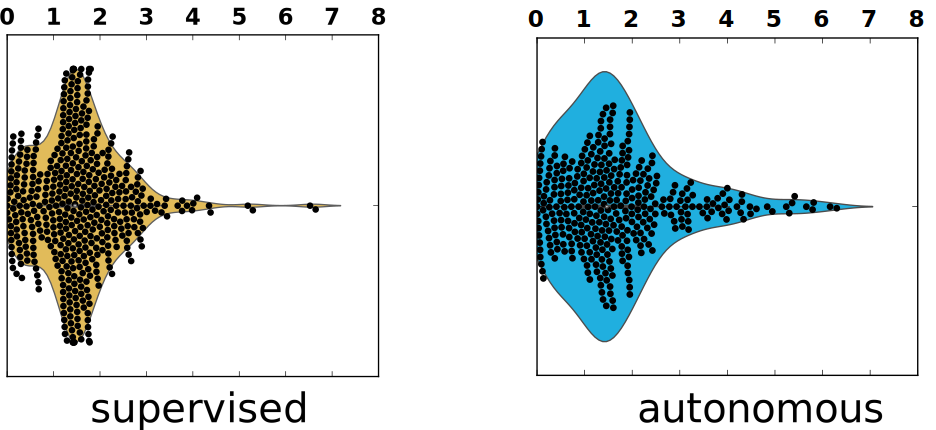
\includegraphics[width=0.9\linewidth]{sparc/social-timing}

        $\rightarrow$ the robot has also learnt an appropriate 'social timing'.
    }

\end{frame}
}

{ \paper{Winkle et al. \textbf{In-Situ Learning from a Domain Expert for Real World Socially Assistive Robot Deployment} RSS 2020}

\begin{frame}{Couch-to-5km: Expert-in-the-loop machine learning}

    \begin{columns}
        \begin{column}{0.5\linewidth}
                \centering
                \includegraphics[height=4cm]{couch25k/hri.jpg}
        \end{column}
        \begin{column}{0.5\linewidth}
                \centering
                \includegraphics[height=4cm]{couch25k/supervised.jpg}
        \end{column}
    \end{columns}

\end{frame}
}

\begin{frame}{Couch to 5km study}
    \begin{itemize}
        \item 9 participants
        \item 3 months; 27 one-hour sessions per participants
        \item 20 input features; 11 actions (task-specific or social)
        \item human-in-loop design and machine learning
        \item robot evolving from full teleoperation to full task and social
            autonomy
    \end{itemize}

\end{frame}

\begin{frame}{Software architecture}
        \centering
        \includegraphics[width=\linewidth]{couch25k/architecture.pdf}

\end{frame}

{
    \paper{Winkle et al. \textbf{In-Situ Learning from a Domain Expert for Real World Socially Assistive Robot Deployment}
    RSS 2020}
    \fullbackground[scale=0.9]{couch25k/finalactiondist.png}
\begin{frame}{Learning to imitate the human expert}
\end{frame}
}
{
    \paper{Winkle et al. \textbf{In-Situ Learning from a Domain Expert for Real World Socially Assistive Robot Deployment}
    RSS 2020}
    \fullbackground[scale=0.9]{couch25k/fullcomp_lbmr.png}
\begin{frame}{Learning to personalise}
\end{frame}
}


\miniframesoff

\begin{frame}{In this lecture}

\begin{itemize}
    \item Basic classifiers: kNNs, SVM, MLP
    \item Build your own emotion classifier from scratch!
%    \item What does the state-of-art look like? Deep graph nets, GANs, Attention
%        nets
    \item ML to teach a robot social behaviours

\end{itemize}

\end{frame}

\begin{frame}{}
    \begin{center}
        \Large
        That's all for today, folks!\\[2em]
        \normalsize
        Questions:\\
        \url{severin.lemaignan@brl.ac.uk} \\[1em]

        Slides:\\
        \href{https://github.com/severin-lemaignan/lecture-hri-ml-for-hri}{\small
        github.com/severin-lemaignan/lecture-hri-ml-for-hri}

    \end{center}
\end{frame}



\end{document}
